\documentclass[10pt,a4paper]{article}
\usepackage[margin=2.6cm]{geometry}
\usepackage[T1]{fontenc}
\usepackage{amsmath,amsthm}
\usepackage{newtxtext,newtxmath}
\usepackage{mathpartir,stmaryrd,microtype,booktabs,enumitem,xcolor}
\usepackage{tikz}
\usepackage[colorlinks,linkcolor=black,citecolor=black,urlcolor=black]{hyperref}

\newtheorem{theorem}{Theorem}
\newtheorem{proposition}[theorem]{Proposition}
\theoremstyle{definition}
\newtheorem{definition}[theorem]{Definition}
\newtheorem{example}[theorem]{Example}
\theoremstyle{remark}
\newtheorem{remark}[theorem]{Remark}

\newcommand{\bx}[1]{\Box_{#1}}
\newcommand{\sem}[1]{\llbracket #1\rrbracket}
\newcommand{\sep}{\mathrel{\#}}
\newcommand{\kw}[1]{\mathsf{#1}}
\newcommand{\keep}{\kw{keep}}
\newcommand{\init}{\kw{init}}
\newcommand{\grow}{\kw{grow}}
\newcommand{\any}{\kw{any}}
\newcommand{\val}{\kw{all\text{-}values}}
\newcommand{\st}{\kw{all\text{-}stores}}
\newcommand{\rigid}{\kw{rigid}}
\newcommand{\fresh}{\kw{fresh}}
\newcommand{\old}{\kw{old}}
\newcommand{\dense}{\kw{dense}}
\newcommand{\every}{\kw{every}}
\newcommand{\apart}{\kw{apart}}
\newcommand{\len}[1]{|#1|}
\newcommand{\tr}[1]{\xrightarrow{#1}}
\newcommand{\resp}{\mathrel{\triangleleft}}
\newcommand{\hoare}[3]{\{#1\}\;#2\;\{#3\}}
\newcommand{\hoarex}[4]{\{#1\}\;#2\;\{#3\mid #4\}}
\newcommand{\code}[1]{\texttt{#1}}
\newcommand{\lean}[1]{\texttt{\small #1}}
\newcommand{\status}[1]{\textsf{\small[#1]}}

\title{Tolerant frames\\[2pt]\large A modal account of fact preservation without ownership}
\author{TScert working note}
\date{11 November 2026}

\begin{document}
\maketitle

\begin{abstract}
\noindent
TypeScript programs are not written against an ownership discipline, and
TScert imposes none; it must still decide which facts about the heap
survive a step. This note gives that reasoning a surface language. Its
one new connective is a modality $\bx{\Phi}F$, ``$F$ holds here and after
any change bounded by the effect $\Phi$'', which stands where the separating
conjunction stands in the frame rule. A fact enters the modality for one
of three reasons: the effect is disjoint from what the fact reads; the
effect changes what the fact reads only in a direction the fact
tolerates; or the invariant annotations on a type fix what the fact reads. Eleven
patterns from a TypeScript code base become one-line annotations, and
four more show what the language still lacks. Every statement carries one of two marks. \status{Lean} names the theorem
of the TScert development that proves the statement's content, and gives
that theorem's scope. \status{conj.} marks a conjecture. A cited Lean theorem states that content directly about heaps and effects; it does not mention $\bx{}$.
\end{abstract}

\section{The problem}

\begin{example}\label{ex:alias}
\code{for (let j = from; j < to; j++) out[j] = xs[j];}\quad
The read is in bounds if $\mathit{to}\le\len{\mathit{xs}}$ holds at each
iteration. The array \code{out} may be an alias of \code{xs}. Since an element write never
shortens an array, the bound survives.
\end{example}

\begin{example}\label{ex:sep}
\code{while (i < flags.length) \{ readRuns(runs); s += flags[i++]; \}}\quad
The callee calls \code{runs.openBrackets.splice(...)}, which may shorten that array. The bound
$i<\len{\mathit{flags}}$ survives the call because the array the callee shortens is
not \code{flags}, and because the field \code{openBrackets} keeps denoting
that array.
\end{example}

Example~\ref{ex:sep} is a frame problem. Example~\ref{ex:alias} is not:
no disjointness is available, and none is required. What the two share is
that the step's \emph{effect} is known and the fact is closed under it.
The language below makes that the primitive.

\section{What exists: variables, locations, stores}\label{sec:model}

Everything below rests on a small inventory, so we state it first.

\paragraph{Variables are not in the heap.} Let $\mathit{Var}$ be the set of variables, ranged over by $x,y$, and
$\mathit{Val}$ the set of values, ranged over by $v$. An environment
$\rho:\mathit{Var}\rightharpoonup\mathit{Val}$ is a finite map from
variables to values.

A local binding of the program (a \code{const}, a \code{let}, a
parameter) is modelled in one of two ways. It is a \emph{cell}, a
location of the heap, when a closure can change it or can see it change:
a closure writes it, or it is written after the creation of a closure
that mentions it. In every other case it is a \emph{variable}, held in $\rho$. Every \code{const} is a variable, and so are most
\code{let}s.

For example, in \code{let i = 0; while (i < k) i++;} the binding
\code{i} is a variable. In \code{let n = 0; const inc = () => \{ n++; \};}
the binding \code{n} is written by a closure, so it is a cell. In
\code{let m = 0; const get = () => m; m = 1;} the binding \code{m} is
written after \code{get} was created, so it is a cell too.

A variable is never updated in place. Programs are taken in a normal
form where each step reads variables and binds one fresh variable; an
assignment \code{x = e} to a variable binds a fresh variable, which the
code after it uses in place of \code{x}. For example, the source assignment
\code{i = i + 1} reads the variable $i_0$ and binds a fresh variable
$i_1$ to $i_0+1$; the code after it reads $i_1$. So a step extends $\rho$ and
changes none of its existing bindings.

Two consequences follow. An effect describes changes to the heap, so no
effect mentions a variable. A fact that mentions only variables, such as
$i<n$, holds after every step once it holds.

\paragraph{Locations.} A heap $h$ is a finite map from locations, ranged over by $l$, to
contents. Locations are natural numbers, and the domain of $h$ is the
initial segment $\{0,\dots,\len h-1\}$: an allocation extends it, and no
location is ever removed. The locations of a heap $h$ are of four kinds, by what they hold. Write
$F$, $C$, $E$ and $S$ for the sets of its locations of each kind; they
partition its domain, $\mathrm{dom}\,h=F\uplus C\uplus E\uplus S$. Each kind belongs to one of two
classes, \emph{value} or \emph{store}; effects refer to locations by
class.

\begin{description}[leftmargin=1.5em,style=nextline]
\item[Field location, in $F$] One for each own key of each object. It
holds the current value of that property. After \code{const o = \{ n: 1, m: 2 \};} the object has two field locations, one for the key \code{n} holding 1 and one for the key \code{m} holding 2; \code{o.n = 3} changes what the first holds and leaves the second. Class: \emph{value}.
\item[Cell, in $C$] One for each local binding that is modelled as a
cell (the previous paragraph) and for each module binding. It holds the
binding's current value. In
\code{let n = 0; const inc = () => \{ n++; \};} the binding \code{n} has
one cell, holding 0; a call \code{inc()} changes what it holds to 1.
Class: \emph{value}.
\item[Element cell, in $E$] One for each present element of each array.
It holds that element's current value. In JavaScript an array literal with nothing between two commas leaves
that index empty: \code{const a = [10, , 30];} makes an array of length
3 with elements at the indices 0 and 2 and none at index 1. An index
with no element is a \emph{hole}. This array has two element cells,
$l_0$ holding 10 and $l_2$ holding 30; the hole at index 1 has no
location. \code{a[0] = 11} changes what
$l_0$ holds. Class: \emph{value}.
\item[Store location, in $S$] One for each array. It holds the array's
\emph{store}: the sequence, in index order, of the array's element cells
and holes. For \code{a} above the store is
$\langle l_0,\circ,l_2\rangle$. \code{a.push(40)} allocates an element
cell $l_3$ and changes the store to $\langle l_0,\circ,l_2,l_3\rangle$;
\code{a.length = 1} changes it to $\langle l_0\rangle$. Class:
\emph{store}.
\end{description}

\noindent
So a heap maps a location to a value or to a store:
$h(l)\in\mathit{Val}$ for $l\in F\cup C\cup E$, and
$h(l)\in\mathit{Store}$ for $l\in S$. Here
$\mathit{Store}=(\mathit{Loc}\uplus\{\circ\})^{*}$ is the set of finite
sequences whose entries are locations or the hole $\circ$, and
$\mathit{Loc}=\mathbb{N}$. For a store
$\sigma=\langle c_0,\ldots,c_{n-1}\rangle$ we write $\len\sigma=n$ for
its length and $\mathit{cells}(\sigma)=\{c_i\mid c_i\ne\circ\}$ for the
set of locations it lists. In one line,
$h:\mathit{Loc}\rightharpoonup\mathit{Val}\uplus\mathit{Store}$.

A value in $\mathit{Val}$ is a scalar, a function, or an object. A
\emph{scalar} is \code{null}, \code{undefined}, a number, a string, a
boolean or a bigint; $\mathit{Scalar}\subseteq\mathit{Val}$ is the set of
scalars and $\mathit{Obj}\subseteq\mathit{Val}$ the set of objects. An object is a finite map $v:\mathit{Key}\rightharpoonup F$ from its
own keys to field locations, fixed when the object is allocated. The
read of a field $f$ of $v$ in a heap $h$ is $h(v(f))$. The object's
identity is the map $v$; what changes is $h$ at the locations $v(f)$. An array is an object with one distinguished field, whose
location $s\in S$ is the array's store location. Its \emph{store} is the
sequence $h(s)=\langle c_0,\dots,c_{n-1}\rangle\in\mathit{Store}$, where
$c_i\in E$ if index $i$ is present and $c_i=\circ$ if it is a hole. The
array's length is $n$, and its element at a present index $i$ is
$h(c_i)$. For \code{const a = [10, , 30];} the store is
$h(s)=\langle l_0,\circ,l_2\rangle$, the length is 3, $h(l_0)=10$ and
$h(l_2)=30$. 
\paragraph{A whole heap.} Take the program
\code{const o = \{ n: 1, m: 2 \}; let k = 0; const inc = () => \{ k++; \}; const a = [10, , 30];}
and number the locations in the order they are allocated. After it runs,
one heap $h$ it can have is:
\[
\begin{array}{llll}
\text{location} & \text{kind} & \text{holds} & \\
0 & F & 1 & \text{the field \code{n} of \code{o}}\\
1 & F & 2 & \text{the field \code{m} of \code{o}}\\
2 & C & 0 & \text{the cell of \code{k}}\\
3 & S & \langle 4,\circ,5\rangle & \text{the store of \code{a}}\\
4 & E & 10 & \text{the element \code{a[0]}}\\
5 & E & 30 & \text{the element \code{a[2]}}
\end{array}
\]
Here $\mathrm{dom}\,h=\{0,\dots,5\}$, $F=\{0,1\}$, $C=\{2\}$, $S=\{3\}$ and $E=\{4,5\}$. The object \code{o} is the map $\{\code{n}\mapsto 0,\ \code{m}\mapsto 1\}$ from its keys to their field locations: the value of \code{o} holds no field contents, and \code{o.n} is read as $h(0)$, \code{o.m} as $h(1)$. The array \code{a} is an object whose distinguished field is the location 3.
The environment $\rho$ holds \code{o}, \code{inc} and \code{a}; the
binding \code{k} is the cell 2. A call \code{inc()} changes $h(2)$ to 1 and nothing else, and \code{o.m = 7} changes $h(1)$ to 7 and nothing else.

So an array has two layers that change independently: the store
$h(s)$, and what each element cell holds. In the example,
\code{a[0] = 11} changes $h(l_0)$ and leaves $h(s)$ as it is, and
\code{a.push(40)} changes $h(s)$ and leaves $h(l_0)$ and $h(l_2)$ as
they are. Each operation writes as follows:

\medskip
\noindent
\begin{tabular}{@{}lll@{}}
\toprule
operation & writes & class written\\
\midrule
\code{x = e}, \code{x} a variable & nothing in the heap & \\
\code{x = e}, \code{x} a cell & the cell & \emph{value}\\
\code{o.f = e} & the field location & \emph{value}\\
\code{a[i] = e}, index present & the element cell & \emph{value}\\
\code{a[i] = e} at a hole or past the end; \code{push} & the store (longer or filled), and a new cell & \emph{store}\\
\code{pop}, \code{splice}, \code{a.length = n} & the store (possibly shorter) & \emph{store}\\
\bottomrule
\end{tabular}
\medskip

\noindent
The \emph{value} class is thus ``contents'': every location that holds
something other than a store. The \emph{store} class is ``shape'': which
elements an array has and how many. A fact about a length or about
presence reads a store; a fact about what a field or an element contains
reads a value location.

\paragraph{Which locations can change.} A location never moves or
disappears; what changes is its contents. We say that a location $l$
\emph{changes} between two heaps $h$ and $h'$ when $h'(l)\ne h(l)$.
Every location can change, through any alias. What bounds the change is the location's
\emph{contract}: the set of contents the location may hold, fixed when
the location is allocated. A field declared \code{n: number} has the
contract ``a number'': \code{o.n = 2} is within it and \code{o.n = "a"}
is outside it. TypeScript's \code{readonly} restricts one view of a
location and makes no location immutable, since another alias may write.

A location is \emph{immutable} exactly when its contract admits a single
value. Two kinds of location are immutable. The first is a field
declared \code{@stable}. This is an annotation of TScert, written in a
comment on a \code{readonly} field of a record type:
\code{type Runs = \{ /** @stable */ readonly openBrackets: number[] \}}.
It states that the field holds, for the object's whole life, the value
the object was created with; the contract of the field's location is
that one value. Here the field \code{openBrackets} of a \code{Runs}
object always holds the same array, whose elements and length may still
change. The second is a typed array's length. They belong to the value
class like any field, and no admissible step (Section~3) changes them.

\section{Model}

\paragraph{Worlds and states.} A \emph{world} $W$ maps each location to
its contract. A contract is a type, and a type denotes a predicate on
contents that is step-indexed and world-monotone~\cite{ahmed}. A world
$W'$ \emph{extends} $W$ when it gives every location of $W$ the contract
$W$ gives it; $W'$ may have more locations.

A heap $h$ \emph{meets} a world $W$ when every location of $h$ holds
contents within its contract in $W$; an environment meets $W$ when each
of its values does. A \emph{state} is a tuple $(\rho,h,W,k)$: an
environment, a heap, a world that $\rho$ and $h$ meet, and a budget
$k>0$ of remaining steps. A
state is \emph{well-formed} when every value in $\rho$ meets its type
and every element cell that a store lists is a location of $h$. In the
heap of Section~2 the store $\langle 4,\circ,5\rangle$ lists the locations 4 and 5, and both are in $\mathrm{dom}\,h$.

A write within a location's contract preserves every typing judgment,
whatever aliases exist~\cite{ahmed}. This is the one use the note makes
of types.

\paragraph{Admissible transitions.} An admissible transition is a change
of state that respects every contract. Its definition mentions no
program. A state $s'=(\rho',h',W',k')$ is \emph{admissible from} a state
$s=(\rho,h,W,k)$ when $W'$ extends $W$ and $k'\le k$. Since $s'$ is a
state, $h'$ meets $W'$; so every location of $h$ holds in $h'$ contents
within the contract it had in $W$. We write $h\tr{}_\rho h'$ when $h$
and $h'$ are the heaps of two such states and $\rho'$ extends $\rho$
\status{Lean: \lean{Admissible}}.

In the heap of Section~2, the call \code{inc()} takes $h$ to the heap
that differs from $h$ only in holding 1 at location 2. The contract of
location 2 is ``a number'', so this is an admissible transition. A heap
holding a string at location 2 is not reached from $h$ by any admissible
transition.

Programs enter through a theorem, not through the definition. Let $t$ be
a term that is safe at a state $s$, in the sense of the step-indexed
model; a term the type system accepts is. If $t$ runs from $s$ for $j$
steps and reaches a heap $h'$, then $h'$ is the heap of a state that is
admissible from $s$, with budget $k-j$
\status{Lean: \lean{run}, \lean{run\_normal}, \lean{run\_throw}, \lean{safe\_run}}.
So what is proved below of every admissible transition holds of every
step, call and callback of typed code.

The relation has four properties, used throughout:
\begin{description}[leftmargin=1.5em,style=nextline]
\item[(T1) Preorder] $h\tr{}_\rho h$; and if $h\tr{}_\rho h'$ and
$h'\tr{}_\rho h''$ then $h\tr{}_\rho h''$, the worlds composing through
the intermediate state's world
\status{Lean: \lean{Admissible.refl}, \lean{Admissible.trans}}.
\item[(T2) Growth] If $h\tr{}_\rho h'$ then $\len h\le\len{h'}$: a
transition allocates and never removes a location
\status{Lean: \lean{Admissible.length\_le}}.
\item[(T3) Fixed objects] Let $v:\mathit{Key}\rightharpoonup F$ be an
object value and $h\tr{}_\rho h'$. The domain of $v$ and each location
$v(f)$ are the same before and after: the field $f$ of $v$ is read as
$h(v(f))$ in $h$ and as $h'(v(f))$ in $h'$. This holds because $v$ is a
value: it does not depend on the heap.
\item[(T4) Immutable locations] If $h\tr{}_\rho h'$, $l<\len h$ and the
contract of $l$ admits the single value $u$, then $h(l)=h'(l)=u$
\status{Lean: \lean{Admissible.stable\_value}}.
\end{description}

\paragraph{Changes.} A \emph{change} bounds how the contents of one
location may differ between two heaps. One of the changes below, $\grow$, must say that the cells a store
newly lists are \emph{new} locations. So a change takes a parameter $b$,
a heap length: a location is new when it is at or above $b$. Formally a
change $\delta$ is a family of preorders $\delta_b$ on contents, one for
each $b\in\mathbb{N}$, with $\delta_{b'}\subseteq\delta_b$ for
$b\le b'$: a larger $b$ leaves fewer locations new, so it allows less.
We write $\delta_b(u,u')$ when $\delta_b$ relates the old contents $u$
to the new contents $u'$.

The parameter is used in two places only. Among the named changes,
condition (iv) of $\grow$ reads it; $\keep$, $\init$, $\kw{scalar}$ and
$\any$ are the same relation for every $b$. And the action of an effect
(below) sets it: a change that starts from a heap $h$ is taken at
$b=\len h$, so ``new'' means allocated by that change. There are five named changes. Recall that
$\mathit{Obj}\subseteq\mathit{Val}$ is the set of objects (Section~2).
Recall that $\mathit{cells}(\sigma)$ is the set of locations a store
$\sigma$ lists. Write $N$ for the maximal array length. For
contents $u,u'$:
\[
\begin{array}{lcl}
\keep_b(u,u') &\iff& u'=u\\[2pt]
\init_b(u,u') &\iff& u'=u\ \vee\ (u\in\{\code{null},\code{undefined}\}\wedge u'\in\mathit{Val})\\[2pt]
\kw{scalar}_b(u,u') &\iff& u'=u\ \vee\ (u\in\mathit{Val}\setminus\mathit{Obj}\wedge u'\in\mathit{Val})\\[2pt]
\grow_b(u,u') &\iff& \kw{scalar}_b(u,u')\ \vee\ (u,u'\in\mathit{Store}\wedge u\preceq_b u')\\[2pt]
\any_b(u,u') &\iff& \kw{true}
\end{array}
\]
where, for two stores, $\sigma\preceq_b\sigma'$ (read: $\sigma'$ is a
\emph{growth} of $\sigma$ at $b$) is the conjunction of four conditions:
\[
\begin{array}{ll}
\text{(i)} & \len\sigma\le\len{\sigma'}\\[2pt]
\text{(ii)} & \forall n.\ \mathit{dense}_n(\sigma)\Rightarrow\mathit{dense}_n(\sigma'),\quad\text{where }\mathit{dense}_n(\sigma)\iff n\le\len\sigma\wedge\forall i<n.\ \sigma_i\ne\circ\\[2pt]
\text{(iii)} & \len\sigma\le N\Rightarrow\len{\sigma'}\le N\\[2pt]
\text{(iv)} & \mathit{cells}(\sigma')\setminus\mathit{cells}(\sigma)\subseteq\{l\mid l\ge b\}.
\end{array}
\]
In words: $\keep$ allows no change. $\init$ lets \code{null} or
\code{undefined} be replaced by any value. $\kw{scalar}$ lets any value
that is not an object (a scalar or a function) be replaced by any value.
$\grow$ also lets a store grow. $\any$ allows everything.

A change bounds contents and ignores types. So
$\kw{scalar}_b(1,\code{"a"})$ holds: a number may become a string as far
as the change is concerned. What forbids it at a location declared
\code{number} is the contract. A change bounded by an effect is, by its
definition below, also an admissible transition, so both bounds apply:
the new contents are related to the old ones by the change, and they are
within the location's contract. For a field declared
\code{n: number | string}, $\kw{scalar}$ allows the step from 1 to
\code{"a"} and so does the contract. For a field declared
\code{n: number} the contract forbids it.

Each change allows all that the one before it allows:
\[
\keep\sqsubseteq\init\sqsubseteq\kw{scalar}\sqsubseteq\grow\sqsubseteq\any .
\]
\status{Lean: \lean{Change.Holds}; \lean{Change.Holds.refl}, \lean{.mono}, \lean{.trans}, \lean{.lower}}

Examples. Let $l$ be the location of \code{c}, holding \code{undefined}. The
assignment in \code{c ??= build()} changes the contents of $l$ from
\code{undefined} to the value $v$ that \code{build()} returns, and
$\init_b(\code{undefined},v)$ holds. The assignment \code{o.n = 3}
changes the contents of the field location of \code{n} from 1 to 3, and
$\kw{scalar}_b(1,3)$ holds. With $b=6$, $\grow_6$ relates the store
$\langle 4,\circ,5\rangle$ to $\langle 4,\circ,5,6\rangle$ (a
\code{push}) and to $\langle 4,6,5\rangle$ (a write at the hole). It
does not relate it to $\langle 4\rangle$, which fails (i), nor to
$\langle 4,\circ,5,0\rangle$, which fails (iv): 0 is an old location.

\paragraph{Regions.} Figure~\ref{fig:heap} shows the heap of Section~2 and the locations that each region defined in this paragraph denotes in it.

\begin{figure}[ht]
\centering
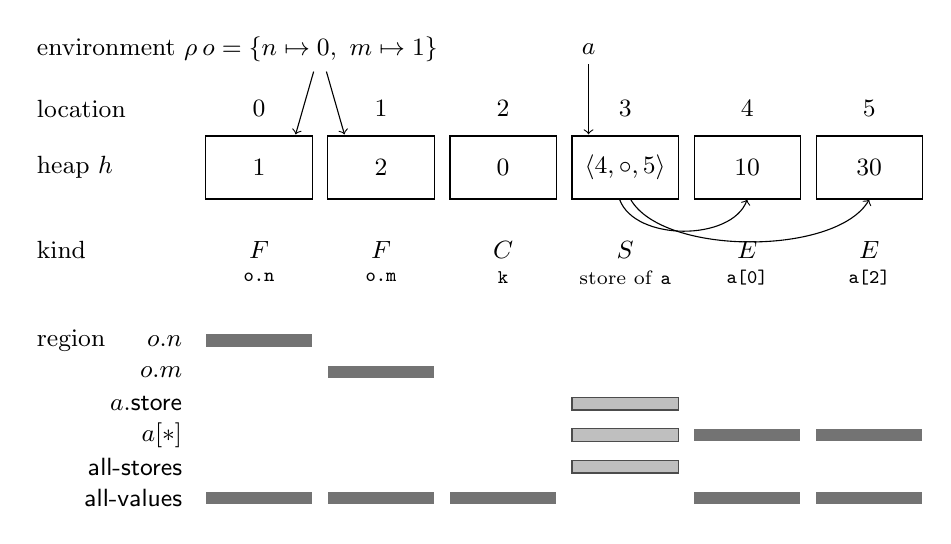
\begin{tikzpicture}[x=1.55cm,y=1cm,font=\small,
  cell/.style={draw,minimum width=1.35cm,minimum height=0.8cm,inner sep=1pt},
  bar/.style={fill=black!55,minimum width=1.35cm,minimum height=0.16cm,inner sep=0pt},
  sbar/.style={bar,fill=black!25,draw=black!70}]
\node[anchor=west] at (-1.9,1.5) {environment $\rho$};
\node[anchor=west] at (-1.9,0.75) {location};
\node[anchor=west] at (-1.9,0) {heap $h$};
\node[anchor=west] at (-1.9,-1.05) {kind};
\node[anchor=west] at (-1.9,-2.2) {region};
\foreach \i/\c/\k/\n in {0/1/F/{\code{o.n}},1/2/F/{\code{o.m}},2/0/C/{\code{k}},3/{$\langle 4,\circ,5\rangle$}/S/{store of \code{a}},4/10/E/{\code{a[0]}},5/30/E/{\code{a[2]}}}{
  \node at (\i,0.75) {\i};
  \node[cell] (c\i) at (\i,0) {\c};
  \node at (\i,-1.05) {$\k$};
  \node[font=\scriptsize] at (\i,-1.4) {\n};
}
\node (o) at (0.5,1.5) {$o=\{n\mapsto 0,\ m\mapsto 1\}$};
\node (a) at (2.7,1.5) {$a$};
\draw[->] (o) -- (0.3,0.42);
\draw[->] (o) -- (0.7,0.42);
\draw[->] (a) -- (2.7,0.42);
\draw[->] ([xshift=-2pt]c3.south) to[out=-70,in=-110,looseness=0.9] (c4.south);
\draw[->] ([xshift=2pt]c3.south) to[out=-60,in=-120,looseness=0.7] (c5.south);
\foreach \y/\name/\cells in {-2.2/{$o.n$}/{0},-2.6/{$o.m$}/{1},-3.0/{$a.\kw{store}$}/{3},-3.4/{$a[\ast]$}/{3,4,5},-3.8/{$\st$}/{3},-4.2/{$\val$}/{0,1,2,4,5}}{
  \node[anchor=east] at (-0.55,\y) {\name};
  \foreach \j in \cells { \ifnum\j=3 \node[sbar] at (\j,\y) {}; \else \node[bar] at (\j,\y) {}; \fi }
}
\end{tikzpicture}
\caption{The heap of Section~2 and what each region denotes in it. Top:
the object \code{o} points to its two field locations, and the array
\code{a} to its store location. Middle: the six locations with their
contents and kinds; the store at location 3 lists the element cells 4
and 5, with a hole between them. Bottom: each bar marks a location the
region denotes; store locations are drawn lighter.}\label{fig:heap}
\end{figure}

A \emph{path} $\pi=x.f_1\ldots f_k$ is a variable
followed by field names. Its \emph{read} in $(\rho,h)$ starts from
$\rho(x)$ and follows the fields $f_1,\ldots,f_k$ in turn through $h$;
the read \emph{fails} when a value on the way is not an object with the
next field. A \emph{region} $r$ denotes a set $r(\rho,h)$ of locations
of $h$. There are five forms:
\begin{description}[leftmargin=1.5em,style=nextline]
\item[{$\st$}] Every location of class store:
$\st(\rho,h)=S$. In the heap of Section~2 it denotes $\{3\}$.
\item[{$\val$}] Every location of class value:
$\val(\rho,h)=F\cup C\cup E$. In the heap of Section~2 it denotes
$\{0,1,2,4,5\}$.
\item[{$\pi.\kw{store}$}] The store location of the one array that $\pi$
reads: $(\pi.\kw{store})(\rho,h)=\{s\}$, where $s$ is that array's store
location. Example: $a.\kw{store}$ denotes $\{3\}$.
\item[{$\pi[\ast]$}] That store location together with the element cells
its store lists: $(\pi[\ast])(\rho,h)=\{s\}\cup\mathit{cells}(h(s))$.
Example: $a[\ast]$ denotes $\{3,4,5\}$.
\item[{$\pi.f$}] The field location for the key $f$ of the one object
$v$ that $\pi$ reads: $(\pi.f)(\rho,h)=\{v(f)\}$. Examples: $o.n$
denotes $\{0\}$ and $o.m$ denotes $\{1\}$.
\end{description}
\noindent
The first two regions are named for what they cover: all the stores of
the heap, and all its value locations. In TScert's \code{Modifies}
annotation they are written \code{stores} and \code{values}. A region at
a path whose read fails denotes the empty set: if \code{z} is
\code{null}, then $z.\mathit{open}.\kw{store}$ denotes $\emptyset$.

\paragraph{Effects.} An \emph{effect} says where a step may change the
heap and by how much. It is a finite set of entries $r:\delta$, each a
region and a change:
\[
\begin{array}{rcl}
\Phi &::=& \{\,r_1:\delta_1,\ \ldots,\ r_k:\delta_k\,\}\\[3pt]
r &::=& \st \mid \val \mid \pi.\kw{store} \mid \pi[\ast] \mid \pi.f\\[3pt]
\delta &::=& \keep\mid\init\mid\kw{scalar}\mid\grow\mid\any
\end{array}
\]
Two examples. The effect $\{\val:\any,\ \st:\grow\}$ reads: every
location that is not a store may change arbitrarily, and every array may
grow and none may shrink. It is the effect of an element write
\code{out[j] = v} whose target array is unknown. The effect
$\{\val:\any,\ y.\kw{store}:\any\}$ reads: every location that is not a
store may change arbitrarily, the one array $y$ may change arbitrarily,
and every other array is unchanged. It is the effect of a call that may
shorten $y$, as \code{y.splice(...)} does.

\paragraph{The action of an effect.} An effect $\Phi$ denotes a relation
$\tr{\Phi}_\rho$ between heaps, its \emph{action}. We say that $h'$ is
reached from $h$ by a change \emph{bounded by} $\Phi$ when
$h\tr{\Phi}_\rho h'$:
\[
h\tr{\Phi}_\rho h'\iff h\tr{}_\rho h'\ \wedge\ \forall l<\len h.\ \bigl(h'(l)=h(l)\ \vee\ \exists (r:\delta)\in\Phi.\ l\in r(\rho,h)\wedge\delta_{\len h}(h(l),h'(l))\bigr).
\]
In words: the transition is admissible; and every location of $h$ either
holds what it held, or lies in the region of some entry and changed
within that entry's change. Three points of the definition matter later.
The regions are read in the heap $h$ the change starts from, as a
dynamic frame is~\cite{kassios}. A location that no entry covers is
unchanged. Locations at or above $\len h$ are allocated by the
transition and are unconstrained.

For example, let $h$ be the heap of Section~2 and let $h'$ be $h$ after
\code{a.push(40)}: $h'(3)=\langle 4,\circ,5,6\rangle$, $h'(6)=40$, and $h'$ agrees with $h$ on 0, 1, 2, 4 and 5. Then $h\tr{\{\st:\grow\}}_\rho h'$:
location 3 is in $\st(\rho,h)$ and changed within $\grow_6$, the locations 0, 1, 2, 4 and 5 are unchanged, and 6 is new. After
\code{a.length = 1} the store is $\langle 4\rangle$, a change that is
not within $\grow$; that transition is bounded by
$\{a.\kw{store}:\any\}$ and is not bounded by $\{\st:\grow\}$.

\paragraph{Order, top, rigidity.} We write $\Phi\sqsubseteq\Psi$ when
the action of $\Phi$ is included in the action of $\Psi$, for every
$\rho$. We write $\top$ for $\{\val:\any,\ \st:\any\}$, the effect of a
step about which nothing is known; every effect is below $\top$.

An effect $\Phi$ is \emph{rigid} when its action is transitive: if
$h\tr{\Phi}_\rho h'$ and $h'\tr{\Phi}_\rho h''$ then
$h\tr{\Phi}_\rho h''$. Rigidity is what lets a fact that survives one
change bounded by $\Phi$ survive any number of them.
\begin{description}[leftmargin=1.5em,style=nextline]
\item[Rigid: class regions] An effect whose regions are $\st$ and $\val$
is rigid at every named change. A change below $\any$ keeps each
location in its class, and $\any$ absorbs any change that follows it.
\item[Rigid: a store at a rigid path] $\{\pi.\kw{store}:\delta\}$ is
rigid on the states where $\pi$ is rigid (Section~4): the path then
reads the same store in $h$ and in $h'$.
\item[Not rigid: cells of a store changed at $\any$]
$\{x[\ast]:\any\}$ is not rigid. A first change may make the store of
$x$ list a location that existed before, such as location 0 in the heap
of Section~2. A second change, whose region is read in the new heap, may
then change location 0, which the region read in $h$ does not contain.
\end{description}

\paragraph{The effect of a command.} The judgment $c:\Phi\mid\Phi^{e}$
states two bounds on a command $c$ run from $(\rho,h)$. If $c$ returns,
in a heap $h'$, then $h\tr{\Phi}_\rho h'$. If $c$ throws, in a heap
$h'$, then $h\tr{\Phi^{e}}_\rho h'$. We write $c:\Phi$ when $\Phi^{e}$ is
$\top$. For example $\code{out[j] = v}:\{\val:\any,\ \st:\grow\}$. This
judgment is what a \code{Modifies} annotation states and what an effect
system derives
\status{Lean: \lean{Post}; \lean{checkRequests\_footprint\_at}, \lean{checkRequests\_regional\_at} for graph code}.

\section{The assertion language}

\paragraph{Syntax.} Assertions $F,G$ are built from atoms $a$:
\[
\begin{array}{rcll}
F,G &::=& a \mid F\wedge G \mid g\vee F \mid \exists v.\,F & g\text{ an invariant assertion; }v\text{ a logical variable}\\
 &\mid& \pi\sep\pi' \mid \apart(x,y) \mid \fresh(x) & \text{separation and freshness}\\
 &\mid& \bx{\Phi}F & \text{the modality}
\end{array}
\]

\paragraph{Atoms.} An atom is a fact of a first-order language over the
heap. An atom is true only where every path it reads is defined. There
are five forms:
\begin{description}[leftmargin=1.5em,style=nextline]
\item[Linear inequality] An inequality between linear terms over
variables and lengths $\len\pi$ of arrays at paths. Examples:
$i<\len{\mathit{flags}}$ and $\mathit{to}\le\len{\mathit{xs}}$.
\item[Equality $\pi\doteq v$] The path $\pi$ reads the value $v$.
Example: $z\doteq\code{null}$.
\item[Density $\dense(x,n)$] The first $n$ indices of the array $x$ are
present. For \code{a = [10, , 30]}, $\dense(a,1)$ holds and $\dense(a,2)$
does not.
\item[Kind of contents] The contents of a cell are of a stated kind,
such as a number or an object. Example: the contents of $x.f$ are a
number.
\item[Bounded quantification $\every(z,t,\varphi)$] Each element of the
array $z$ at an index below $t$ satisfies $\varphi$. For
\code{a = [10, , 30]}, $\every(a,1,v>0)$ holds.
\end{description}

\paragraph{Satisfaction.} An assertion is interpreted at a triple
$(\rho,m,h)$: an environment, an \emph{entry mark}, and a heap. The
entry mark $m\le\len h$ is the length the heap had when the current
function invocation started; the locations at or above $m$ are the ones
the invocation has allocated. We write $\rho,m,h\models F$. Atoms read
$\rho$ and $h$ only, and the connectives $\wedge$, $\vee$, $\exists$
have their usual meaning. The other four forms are:
\[
\begin{array}{lcl}
\rho,m,h\models\pi\sep\pi' &\iff& \pi\text{ and }\pi'\text{ read arrays with different store locations},\\[2pt]
\rho,m,h\models\apart(x,y) &\iff& x\sep y\text{, and the stores of }x\text{ and }y\text{ list no common element cell},\\[2pt]
\rho,m,h\models\fresh(x) &\iff& \text{the store location of }\rho(x)\text{ is at or above }m,\\[2pt]
\rho,m,h\models\bx{\Phi}F &\iff& \text{for all }h'\text{, if }h\tr{\Phi}_\rho h'\text{ then }\rho,m,h'\models F .
\end{array}
\]
So $\bx{\Phi}F$ says: $F$ holds in every heap reached from here by a
change bounded by $\Phi$. Since $h\tr{\Phi}_\rho h$, it says in
particular that $F$ holds here.

Two examples, in the heap $h$ of Section~2, where $\len a=3$. First,
$\rho,m,h\models\bx{\val:\any,\ \st:\grow}(3\le\len a)$: a change bounded
by this effect leaves the store of $a$ or grows it, so its length stays
at least 3. Second,
$\rho,m,h\not\models\bx{a.\kw{store}:\any}(3\le\len a)$: the heap after
\code{a.length = 1} is reached by a change bounded by this effect, and
there $\len a=1$. In a function \code{f() \{ const xs = [1]; \ldots \}},
$\fresh(\mathit{xs})$ holds after the declaration: the store of
\code{xs} was allocated by this invocation.

Assertions describe the whole heap. They can be duplicated, and holding
one confers no permission to write.

\paragraph{Invariant assertions and rigid paths.} Two abbreviations:
\[
F\text{ is \emph{invariant}}\ \triangleq\ F\vdash\bx{\top}F
\qquad\qquad
\rigid(\pi)\ \triangleq\ \exists v.\ \bx{\top}(\pi\doteq v) .
\]
An invariant assertion, once true, is true after every admissible
transition. A fact about variables alone, such as $i<n$, is invariant.
So is $x\sep y$ for two variables: an array's store location is fixed
when the array is allocated. A path is rigid when it reads the same
value after every admissible transition. A path through fields whose
contracts admit one value is rigid: \code{runs.openBrackets} is rigid
when \code{openBrackets} is declared \code{@stable}. In $\rigid(\pi)$
the witness $v$ is a logical variable, so it is the same value before
and after the change.

\begin{remark}[Reading]
$\bx{\Phi}F$ is the weakest liberal precondition of $F$ for the command
that makes one arbitrary admissible change bounded by $\Phi$:
$\bx{\Phi}F=\mathit{wlp}(\kw{havoc}\,\Phi,F)$, the reading a verifier
gives a call when it replaces it by its \code{modifies} clause. For a
rigid $\Phi$ it is the weakest assertion that is stronger than $F$ and
stable under $\tr{\Phi}$: the floor of explicit
stabilisation~\cite{wickerson}, at a rely denoted by an effect.
\end{remark}

\begin{proposition}[Laws]\label{prop:laws}\status{conj.}
\begin{enumerate}[label=(\alph*),itemsep=1pt,topsep=2pt]
\item $\bx{\Phi}F\vdash F$.
\item $\bx{\Phi}(F\wedge G)\dashv\vdash\bx{\Phi}F\wedge\bx{\Phi}G$; if $F\vdash G$ then $\bx{\Phi}F\vdash\bx{\Phi}G$.
\item If $\Phi\sqsubseteq\Psi$ then $\bx{\Psi}F\vdash\bx{\Phi}F$.
\item $g\vee\bx{\Phi}F\vdash\bx{\Phi}(g\vee F)$ for invariant $g$.
\item $\bx{\Phi}F\vdash\bx{\Phi}\bx{\Phi}F$ for rigid $\Phi$.
\end{enumerate}
\end{proposition}
\noindent
In words: (a) what holds after every change holds now; (b) the modality
distributes over conjunction and is monotone; (c) a fact that survives a
larger effect survives a smaller one; (d) an invariant disjunct can be
moved under the modality; (e) under a rigid effect, a fact that survives
one change survives a change after a change. Each is immediate: (a) from
reflexivity of the action, (b), (c) and (d) from the definitions, (e)
from transitivity. For effects over class regions
transitivity is \lean{Closed.Holds.trans\_on}; for a store at a path it
is \lean{ArgumentStoreRegionsWithin.trans}, under that theorem's premise
that the path resolves to the same store in both heaps.

\section{Entering the modality}

A fact enters the modality by naming what it reads and how much change
of it the fact tolerates.

\begin{definition}[Support]
A \emph{support} for an assertion $F$ is a finite set $S$ of pairs
$r:\delta$, a region and a change, with this property: for all
$\rho,m,h,h'$, if $\rho,m,h\models F$, $h\tr{}_\rho h'$, and every
location $l<\len h$ in a region $r(\rho,h)$ of a pair $(r:\delta)\in S$
satisfies $\delta_{\len h}(h(l),h'(l))$, then $\rho,m,h'\models F$.
Locations outside the regions of $S$ may change in any admissible way.
\end{definition}

\noindent
For example $\{x.\kw{store}:\grow\}$ supports $n\le\len x$: the fact
reads the store of $x$ and nothing else in the heap, and it tolerates
any growth of that store.

\begin{definition}[Respect]
Let $K$ be an assertion. An effect $\Phi$ \emph{respects} a support $S$
under $K$, written $\Phi\resp_K S$, when for every pair
$(r:\delta)\in S$ and every entry $(r':\gamma)\in\Phi$, either
$\gamma\sqsubseteq\delta$, or $K$ entails that $r$ and $r'$ denote
disjoint sets.
\end{definition}

\noindent
For example $\{\val:\any,\ \st:\grow\}$ respects
$\{x.\kw{store}:\grow\}$ under $\kw{true}$. The entry $\st:\grow$ meets
the first condition, $\grow\sqsubseteq\grow$. The entry $\val:\any$
meets the second: a store location is no location of class value.

\begin{theorem}[Tolerant frame]\label{thm:frame}
If $S$ supports $F$ and $\Phi\resp_K S$, then $K\wedge F\vdash\bx{\Phi}F$.
\status{Lean: \lean{stable\_sound}, with \lean{frame\_sound} for the supports of cell, link, density and element-kind facts}
\end{theorem}
\begin{proof}
Let $h\tr{\Phi}_\rho h'$ and $l\in r(\rho,h)$ with $(r:\delta)\in S$.
Either $h'(l)=h(l)$, and $\delta$ is reflexive, or some
$(r':\gamma)\in\Phi$ covers $l$ and bounds its change by $\gamma$. Then
$r$ and $r'$ are not disjoint, so $\gamma\sqsubseteq\delta$.
\end{proof}

The theorem has two known rules as its extreme cases. When every change
in the support is $\keep$, the condition is that the regions a command
writes are disjoint from the regions a formula reads: the frame rule of
region logic~\cite{bnr}. When $K$ separates no pair, the condition is
that the assertion is stable under an interfering action~\cite{jones}.
The theorem chooses between the two at each pair.

A fact may have several supports and none of them greatest. On
well-formed arrays, $\apart(x,y)$ is supported by
$\{x[\ast]:\grow,\ y[\ast]:\keep\}$: a store that grows lists only the
cells it listed and new ones. It is also supported by the mirror image,
$\{x[\ast]:\keep,\ y[\ast]:\grow\}$. It is not supported by
$\{x[\ast]:\grow,\ y[\ast]:\grow\}$: both stores may come to list the
same new cell.

\begin{proposition}[Axioms of the atoms]\label{prop:axioms}
For variables $x,y,z,w$, a rigid effect in \textsc{(Rigid)}, and $a$ an
atom that reads, besides variables, only what is displayed:
\[
\begin{array}{ll}
\textsc{(Grow)} & n\le\len x\ \vdash\ \bx{\val:\any,\ \st:\grow}\,(n\le\len x)\\[2pt]
\textsc{(Dense)} & \dense(x,n)\ \vdash\ \bx{\val:\any,\ \st:\grow}\,\dense(x,n)\\[2pt]
\textsc{(Sep)} & x\sep y\wedge a(\len x)\ \vdash\ \bx{\val:\any,\ y.\kw{store}:\any}\ a(\len x)\\[2pt]
\textsc{(Every)} & \apart(x,z)\wedge\every(z,t,\varphi)\ \vdash\ \bx{x[\ast]:\any}\,\every(z,t,\varphi)\quad t\text{ a variable, }\varphi\text{ over scalars}\\[2pt]
\textsc{(Init)} & a(\len\pi)\ \vdash\ \bx{\val:\init}\ a(\len\pi)\quad\pi\text{ through fields holding objects}\\[2pt]
\textsc{(Rigid)} & \rigid(\pi)\wedge a(\len{\pi})\ \vdash\ \bx{\Phi}\,a(\len\pi)\quad\text{if } a(\len y)\vdash\bx{\Phi}\,a(\len y)\text{ for a fresh }y\\[2pt]
\textsc{(View)} & a(\kw{view}(w))\ \vdash\ \bx{\top}\,a(\kw{view}(w))\quad\kw{view}(w)\text{ a typed array's length}
\end{array}
\]
\end{proposition}
\noindent
Each axiom, in words, with the Lean theorem that proves its content. The
Lean development proves each for the steps TScert has, not for an
arbitrary transition bounded by the displayed effect.
\begin{description}[leftmargin=1.5em,style=nextline]
\item[\textsc{(Grow)}] A lower bound on a length survives any change
that only grows arrays. It mentions no separation: it is
Example~\ref{ex:alias}. Lean: \lean{termValue\_grown}, for defined terms
on preserved paths.
\item[\textsc{(Dense)}] A dense prefix survives any change that only
grows arrays. Lean: \lean{dense\_support}.
\item[\textsc{(Sep)}] A fact about the length of $x$ survives an
arbitrary change of another array $y$. It is Example~\ref{ex:sep}. Lean:
\lean{regionFirst\_kept}, at a call.
\item[\textsc{(Every)}] A fact about each element of $z$ survives an
arbitrary change of an array $x$ that shares no element cell with $z$.
Lean: \lean{writeAtoms\_holds}, for an element write at a checked index.
\item[\textsc{(Init)}] A fact about a length survives a change that only
initialises: $\init$ changes no location that holds an object, a number
or a store. It is Theorem~\ref{thm:frame} at a support that tolerates
$\init$ on the fields of the path. Lean: \lean{ofClosed\_holds}.
\item[\textsc{(Rigid)}] A fact that holds of an array named by a
variable holds of the array at a rigid path. The substitution of the
witness for $y$ is capture-avoiding. Lean: \lean{stableFirst\_frame},
for \code{@stable} fields on normal return.
\item[\textsc{(View)}] A fact about a typed array's length survives
every change: that length is an immutable location, by (T4). Lean: the
rule \code{view-stable}.
\end{description}

\section{Programs}

\paragraph{Triples.} A triple $\hoarex PcQ{Q^{e}}$ states partial
correctness of a command $c$. If $c$ runs from a state satisfying $P$
and returns, the state it returns in satisfies $Q$. If it throws, the
state at its handler satisfies $Q^{e}$. We write $\hoare PcQ$ when
$Q^{e}$ is $\kw{true}$. For example
$\hoare{\kw{true}}{x=\code{[]}}{\len x=0}$.

The posts $Q$ and $Q^{e}$ are \emph{two-state}: in them $\old(e)$
denotes the value of $e$ in the environment and heap that $c$ started
in. For example \code{x.push(v)} has the post
$\len x=\old(\len x)+1$.

The variable that a step binds is fresh (Section~2). So an assertion $R$
over the variables in scope before $c$ is unaffected by the binding.

\paragraph{Rules.}
\begin{mathpar}
\inferrule*[left=Frame]{\hoarex PcQ{Q^{e}} \\ c:\Phi\mid\Phi^{e}}{\hoarex{P\wedge\bx{\Phi}R\wedge\bx{\Phi^{e}}R^{e}}{c}{Q\wedge R}{Q^{e}\wedge R^{e}}}
\and
\inferrule*[left=Frame$^{+}$]{\hoare PcQ \\ c:\Phi \\ \Phi\text{ rigid}}{\hoare{P\wedge\bx{\Phi}R}{c}{Q\wedge\bx{\Phi}R}}
\and
\inferrule*[left=Loop]{\hoare{I}{c}{I} \\ c:\Phi \\ \Phi\text{ rigid}}{\hoare{I\wedge\bx{\Phi}R}{\code{loop}\ c}{I\wedge\bx{\Phi}R}}
\and
\inferrule*[left=Call]{f(\vec p):\hoare PfQ:\Phi}{\hoare{P[\vec x/\vec p]\wedge\bx{\Phi[\vec x/\vec p]}R}{y=f(\vec x)}{Q[\vec x/\vec p]\wedge R}}
\and
\inferrule*[left=Alloc]{x\text{ fresh} \\ y\text{ ranges over the arrays in scope}}{\hoare{\kw{true}}{x=\code{[]}}{\fresh(x)\wedge\len x=0\wedge\textstyle\bigwedge_y\apart(x,y)}}
\and
\inferrule*[left=Seq-Eff]{c_1:\Phi \\ c_2:\Psi \\ \Psi\rightsquigarrow_{\mathit{ev}}\Psi' \\ \Phi\cup\Psi'\sqsubseteq\Phi}{c_1;c_2:\Phi}
\and
\inferrule*[left=Fresh-Eff]{c:\Phi\cup\{x.\kw{store}:\delta\} \\ \fresh(x)\text{ holds before }c}{c:\Phi\ \text{ from the entry}}
\end{mathpar}

\noindent
The rules one by one:
\begin{description}[leftmargin=1.5em,style=nextline]
\item[\textsc{Frame}] The frame rule, with $\wedge\,\bx{\Phi}$ where
separation logic has $\ast$: a fact $R$ that survives every change
bounded by the effect of $c$ holds after $c$. Its soundness is the
definition of the modality and of $c:\Phi\mid\Phi^{e}$. It holds for a
compound $c$ whose effect is stated at its entry, with the variables $c$
binds renamed apart from those of $R$ and $\Phi$.
\item[\textsc{Frame}$^{+}$] For a rigid effect the frame keeps its
modality after $c$, by law (e).
\item[\textsc{Loop}] As \textsc{Frame}$^{+}$, for any number of
iterations. Here $c$ is one iteration together with the evaluation of
its guard; every exit leaves from a state satisfying $I$; the values the
loop carries from one iteration to the next are variables of $I$; and
$R$ mentions none of them.
\item[\textsc{Call}] The frame rule at a call. The actual arguments
$\vec x$ are variables, hence fixed values. The substitution
$[\vec x/\vec p]$ is capture-avoiding, and $Q$ may mention the result
$y$.
\item[\textsc{Alloc}] A new array is fresh, empty, and apart from every
well-formed array $y$ that exists before the step. These separations are
facts of the state after the step. Later steps keep or lose them like
any other fact.
\item[\textsc{Seq-Eff}] The effect of a sequence, stated at the entry of
the sequence. The effect $\Psi$ of the second command is read where that
command starts, so it is first \emph{rebased} to the entry (below).
\item[\textsc{Fresh-Eff}] A change to an array that the command itself
allocated is no part of the command's effect, seen from its entry.
\end{description}

\begin{definition}[Rebasing]
Let $\Psi$ be an effect read at an intermediate heap and $\Psi'$ an
effect read at the entry heap. $\Psi\rightsquigarrow_{\mathit{ev}}\Psi'$
holds when every location of the entry heap that $\Psi$ covers at a
change $\delta$ is covered by $\Psi'$ at $\delta$ or at a wider change.
The evidence $\mathit{ev}$ records, for each value that $\Psi$ names,
the entry path it was read from, and that this path reads the same in
both heaps.
\end{definition}

\noindent
Three cases follow from the definition. A region at a rigid path rebases
to itself. The store of a fresh array is no location of the entry heap,
so its entry rebases to nothing: this is \textsc{Fresh-Eff}. Any other
region, and the cells of a fresh store, widen to their class. For
example, in \code{f(o) \{ const xs = o.items; xs.push(1); \}} the push
has the effect $\{\mathit{xs}.\kw{store}:\grow\}$ where it starts. If
$o.\mathit{items}$ is rigid, the effect of \code{f} at its entry is
$\{o.\mathit{items}.\kw{store}:\grow\}$. Otherwise it widens to
$\{\st:\grow\}$
\status{Lean: \lean{Post.compose\_at}, \lean{rebaseAll}, \lean{rebase\_sound}, \lean{checkFresh\_sound}}.

\begin{example}[Freshness bounds effects, not facts]\label{ex:fresh}
Let \code{shrink(xs)} pop its argument,
$\code{shrink}:\{\val:\any,\ \mathit{xs}.\kw{store}:\any\}$, and
\code{f() \{ const xs = [1]; shrink(xs); return xs[0]; \}}.
By \textsc{Fresh-Eff}, $\code{f}:\{\val:\any\}$: a caller of \code{f}
sees no change to any array. Inside \code{f} the fact
$0<\len{\mathit{xs}}$ is not derivable under
$\bx{\mathit{xs}.\kw{store}:\any}$, so it does not hold after the call
\code{shrink(xs)}, and the read \code{xs[0]} is refused. Freshness gives
separations, by \textsc{Alloc}. It does not put any fact under a
modality.
\end{example}

\begin{proposition}[Reliance]\label{prop:rely}
Let a native operation alternate its own steps with calls of callbacks,
every one of effect bounded by a rigid $\Phi$, and observe the heap only
between them. If $\bx{\Phi}F$ holds when it starts, $F$ holds at each
observation.
\status{Lean: \lean{rely\_chain}; \lean{map\_rely}, \lean{elems\_rely} for \code{map}}
\end{proposition}
\noindent
For example take \code{xs.map(f)}, where \code{map} reads
$n=\len{\mathit{xs}}$ once at its start. Let $F=\dense(\mathit{xs},n)$
and $\Phi=\{\val:\any,\ \st:\grow\}$. If \code{f}, with all it calls,
has an effect bounded by $\Phi$, then by \textsc{(Dense)} and the
proposition $F$ holds each time \code{map} reads an element. So the
result of \code{xs.map(f)} is dense when \code{xs} is.

\paragraph{Exact posts.} A step may state an exact two-state relation,
such as $\len x=\old(\len x)+1$ for \code{x.push(v)}. This is a strong
update on shared state, and it needs no ownership. The post constrains
the written location only. Every other fact crosses the step by
\textsc{Frame}, and that rule accounts for aliasing. For example, let
$y$ be an array that may be $x$. After \code{x.push(v)} the lower bound
$n\le\len y$ still holds, by \textsc{(Grow)}. The equality $\len y=n$
does not: it is false when $y$ is $x$.

\section{Transfer along edges}\label{sec:transfer}

A node of a control-flow graph has one \emph{exit edge} for each way it
completes: a normal return, each branch it can take, and a throw to a
handler. An exit edge $e$ carries four things:
\begin{description}[leftmargin=1.5em,style=nextline]
\item[The effect $\Phi_e$] The effect of the node when it completes
through $e$.
\item[The post $Q_e$] A sound two-state post of the node on that exit.
It includes the binding of the result, or of the thrown value.
\item[The condition $B_e$] The condition under which a branch is taken;
$\kw{true}$ on other edges.
\item[The renaming $\theta_e$] A map from the variables of the node to
the variables of the target of $e$.
\end{description}
\noindent
In Example~\ref{ex:full} below, the true exit of the test
\code{j < to} has $\Phi_e=\emptyset$, $B_e=(j<\mathit{to})$ and the
identity renaming; the back edge has $\theta_e=[j\mapsto j']$.

The \emph{knowledge} $\Sigma$ at a point of the graph is a finite set of
assertions. A state $s$ satisfies it at an entry mark $m$, written
$s\models_m\Sigma$, when it satisfies each of them.

\begin{definition}[Checked transfer]
$\mathrm{Check}(c,\Sigma,e,A)$ holds when there is a finite set
$K_e\subseteq\Sigma$ with a derivation of $\Sigma\vdash\bx{\Phi_e}F$ for
each $F\in K_e$, and a derivation of
\[
\old(\Sigma)\ \wedge\ Q_e\ \wedge\ B_e\ \wedge\ K_e\ \ \vdash\ \ \theta_e^{*}A ,
\]
where $\old(\Sigma)$ is $\Sigma$ at the node's entry state,
$\theta_e^{*}A$ is $A$ with the target's variables replaced by the
node's, and the entailment includes that every path $A$ reads is
defined.
\end{definition}

\begin{theorem}[Transfer]\label{thm:transfer}\status{conj.\ as one statement; proved for TScert's checker edge by edge, \lean{ControlFlow} with \lean{HeapKnowledge}'s transport}
If $s$ is well-formed, $s\models_m\Sigma$, the node $c$ runs from $s$
through exit $e$ to $s'$, and $\mathrm{Check}(c,\Sigma,e,A)$, then
$\theta_e(s')\models_m A$.
\end{theorem}
\noindent
The proof is \textsc{Frame} for $K_e$ and consequence for the rest. The
entry mark $m$ is fixed for the invocation, and $\old$ refers to the
state at the entry of the node.

\paragraph{Sound graphs.} Annotate each point of a graph with knowledge.
The annotated graph is \emph{sound} when its entry state satisfies the
knowledge at the entry, and $\mathrm{Check}$ holds on every edge against
the knowledge at the edge's target. Merges and loop heads are targets
like any other.

\paragraph{The forward pass.} A forward pass is a way of
\emph{computing} annotations that satisfy these checks. At a node it
keeps the facts it can derive under the modality, and adds what the post
gives. At a merge it keeps what every incoming edge establishes. At a
loop head one pass cannot compute the knowledge: the knowledge is
supplied, and checked on the back edges like on any other edge.

The derivations are those of Propositions~\ref{prop:laws}
and~\ref{prop:axioms} together with linear arithmetic. The system is
sound. It is deliberately incomplete for semantic entailment.

\begin{example}[Example~\ref{ex:alias}, in full]\label{ex:full}
With the loop variable a parameter of the head, and
$\Sigma_H(j)=\{0\le j,\ \mathit{to}\le\len{\mathit{xs}}\}$:
\[
\begin{array}{llll}
 & \text{node or edge} & \text{effect} & \text{obligation and its reason}\\[2pt]
1 & \text{entry}\to H(\mathit{from}) & & 0\le\mathit{from},\ \mathit{to}\le\len{\mathit{xs}}\ \text{given}\\
2 & H(j):\ \code{j < to}\ \text{true} & \emptyset & B=(j<\mathit{to});\ \text{all of }\Sigma_H\text{ kept, }\emptyset\text{ changes nothing}\\
3 & v=\code{xs[j]} & \emptyset & \text{the read: }0\le j<\mathit{to}\le\len{\mathit{xs}}\\
4 & \code{out[j] = v} & \val{:}\any,\ \st{:}\grow & \mathit{to}\le\len{\mathit{xs}}\ \text{by \textsc{(Grow)}};\ 0\le j,\ j<\mathit{to}\ \text{invariant}\\
5 & j'=j+1 & \emptyset & Q=(j'=j+1)\\
6 & \text{back edge},\ \theta=[j\mapsto j'] & & \theta^{*}\Sigma_H=\{0\le j',\ \mathit{to}\le\len{\mathit{xs}}\}\ \text{from }0\le j,\ Q,\ \text{row 4}\\
7 & H(j):\ \code{j < to}\ \text{false} & \emptyset & \text{exit with }\Sigma_H\wedge\neg(j<\mathit{to})
\end{array}
\]
No row mentions whether \code{out} is an alias of \code{xs}.

Now suppose the invariant also had an upper bound,
$\len{\mathit{xs}}\le n$. Row 4 loses it. No axiom puts an upper bound
under $\bx{\st:\grow}$, and the bound is false after the write when
\code{out} is \code{xs} and $j=\len{\mathit{xs}}$.

The upper bound is kept under two additions. The knowledge $\Sigma_H$
includes $\apart(\mathit{out},\mathit{xs})$. And the effect of the write
is stated at its region, $\{\mathit{out}[\ast]:\grow\}$. Then the bound
is kept by \textsc{(Sep)}. The separation itself becomes an obligation
of rows 1 and 6.
\end{example}

\section{The patterns}

\noindent
\begin{tabular}{@{}p{0.25\textwidth}p{0.71\textwidth}@{}}
\toprule
Lower bound under aliasing (Ex.~\ref{ex:alias}) & $\mathit{to}\le\len{\mathit{xs}}\vdash\bx{\val:\any,\,\st:\grow}(\mathit{to}\le\len{\mathit{xs}})$\hfill\textsc{(Grow)}\\[2pt]
Bound across a rewriting call (Ex.~\ref{ex:sep}) & $\mathit{flags}\sep y\wedge i<\len{\mathit{flags}}\vdash\bx{\val:\any,\,y.\kw{store}:\any}(i<\len{\mathit{flags}})$, $y$ standing for the rigid $\mathit{runs}.\mathit{openBrackets}$\hfill\textsc{(Sep)}, \textsc{(Rigid)}\\[2pt]
Storage the function allocated & the write is no part of the function's effect; $\apart(x,y)$ for older $y$\hfill\textsc{Fresh-Eff}, \textsc{Alloc}\\[2pt]
Write-once cache, \code{c ??= build()} & $a\vdash\bx{\Phi_{\mathit{build}}\cup\{\val:\init\}}\,a$, by Theorem~\ref{thm:frame} at a support respected by $\Phi_{\mathit{build}}$ and tolerating $\init$\hfill\textsc{(Init)}\\[2pt]
Reliance during callbacks & $\dense(\mathit{xs},n)\vdash\bx{\val:\any,\,\st:\grow}\dense(\mathit{xs},n)$\hfill Prop.~\ref{prop:rely}\\[2pt]
Quantified fact across a write & $\apart(a,z)\wedge\every(z,t,\varphi)\vdash\bx{a[\ast]:\any}\every(z,t,\varphi)$\hfill\textsc{(Every)}\\[2pt]
Structures built in step & $\hoare{\len a=\len b\wedge a\sep b}{\code{a.push(v)}}{\len a=\old(\len a)+1\wedge\len b=\old(\len b)}$\hfill post, \textsc{(Sep)}\\[2pt]
Separation where a value exists & $(z\doteq\code{null}\vee\mathit{xs}\sep z.\mathit{open})\wedge a(\len{\mathit{xs}})\vdash\bx{\val:\any,\,z.\mathit{open}.\kw{store}:\any}\,a(\len{\mathit{xs}})$; at \code{null} the region is empty\\[2pt]
Fact through a field & $\rigid(x.f)\wedge n\le\len{x.f}\vdash\bx{\val:\any,\,\st:\grow}(n\le\len{x.f})$; fails without $\rigid$\hfill\textsc{(Rigid)}\\[2pt]
Typed-array length & $i<\kw{view}(w)\vdash\bx{\top}(i<\kw{view}(w))$\hfill\textsc{(View)}\\[2pt]
Fact at a handler & $\bx{\Phi^{e}}R^{e}$\hfill\textsc{Frame}\\
\bottomrule
\end{tabular}

\medskip
Four patterns are outside the language. Three need a form it lacks:
\begin{description}[leftmargin=1.5em,style=nextline]
\item[A fact about a field of each element] Example:
$\code{rows[i].n}\ge 0$ for every $i$. It needs a region $z[\ast].n$: a
path from each element cell the store lists.
\item[Overlapping typed-array views] Two views are distinct objects over
one buffer, so $\sep$ on their stores says nothing about their elements.
They need regions of buffer cells with offsets.
\item[A callback that writes what it captured] Example:
\code{walk(xs, v => out.push(v))}. Each use has a closed effect. A
reusable specification of \code{walk} needs an effect variable,
$\forall\varepsilon.\ \Phi\cup\varepsilon$.
\end{description}
\noindent
The fourth needs no new form. It needs a separation that the rules do
not establish:
\begin{description}[leftmargin=1.5em,style=nextline]
\item[A record replaced on each loop pass] The new record must be
separated from the loop's iterator on every back edge. \textsc{Alloc}
states separation only against what is in scope at the allocation.
\end{description}

\section{Relation to separation logic}

The language takes from separation logic~\cite{ohearn} the frame rule
and, in \textsc{Alloc} and \textsc{Fresh-Eff}, the principle that what a
computation allocates is outside every frame of its callers. It has no
separating conjunction and no resource model: assertions describe the
whole heap and are duplicable. In \textsc{Frame} the effect is stated,
where separation logic derives a command's footprint from its
precondition; in return the modality frames facts that overlap what the
command writes. A precise correspondence would embed assertions about a
subheap into assertions about the whole heap and relate $P\ast R$ to
$\bx{\Phi}R$ for the effect $\Phi$ confined to $P$'s subheap; we state
none. Whether the model is an instance of abstract separation
logic~\cite{coy} or of Views~\cite{views} is open; it would need a
composition on supports.

The closest relatives are region logic and dynamic frames, for effects
as region expressions read in the pre-state; rely/guarantee with explicit
stabilisation, for the modality; and monotone state~\cite{adr,ahman},
for $\init$ and $\grow$, which here are enforced by the effect judgment
and by no resource discipline.

\paragraph{How much separation.} In these patterns: pairwise
disjointness of single stores ($\sep$), and of a store with its cells
($\apart$) where a fact reads element contents, each established by
allocation or assumed at a function's entry. Five of the eleven
obligations use none. This describes the patterns met so far and is no
completeness claim.

\section{Limits}\label{sec:limits}

\begin{description}[leftmargin=1.5em,style=nextline]
\item[Effects are closed] An effect has no variables. So a higher-order
function states one bound for every callback it admits~\cite{bty}.
\item[Await] Across an \code{await} the effect is that of the
environment, $\top$.
\item[Broken and restored invariants] An invariant that a callee breaks
and then restores has no form. At each step a fact either enters the
modality or is derived anew.
\item[Fixed contracts] A location's contract never changes, so there is
no type-changing update.
\item[Transfer as one Lean theorem] The laws and rules are stated for
admissible transitions and use the properties (T1) to (T4) of Section~3.
Theorem~\ref{thm:transfer} is not one Lean theorem. Stating it in Lean
needs, beyond those properties, the correspondence between this note's
named variables and the model's environment, which a result extends by a
push.
\end{description}

\begin{thebibliography}{9}\small\itemsep1pt
\bibitem{ahmed} A.~Ahmed. \emph{Semantics of Types for Mutable State}. PhD thesis, Princeton University, 2004.
\bibitem{adr} A.~Ahmed, D.~Dreyer, A.~Rossberg. State-dependent representation independence. POPL 2009.
\bibitem{ahman} D.~Ahman, C.~Fournet, C.~Hri\c{t}cu, K.~Maillard, A.~Rastogi, N.~Swamy. Recalling a witness: foundations and applications of monotonic state. PACMPL 2(POPL), 2018.
\bibitem{bnr} A.~Banerjee, D.~Naumann, S.~Rosenberg. Local reasoning for global invariants, part I: region logic. J.~ACM 60(3), 2013.
\bibitem{bty} L.~Birkedal, N.~Torp-Smith, H.~Yang. Semantics of separation-logic typing and higher-order frame rules. LICS 2005.
\bibitem{coy} C.~Calcagno, P.~O'Hearn, H.~Yang. Local action and abstract separation logic. LICS 2007.
\bibitem{views} T.~Dinsdale-Young, L.~Birkedal, P.~Gardner, M.~Parkinson, H.~Yang. Views: compositional reasoning for concurrent programs. POPL 2013.
\bibitem{jones} C.~B.~Jones. Tentative steps toward a development method for interfering programs. ACM TOPLAS 5(4), 1983.
\bibitem{kassios} I.~Kassios. Dynamic frames: support for framing, dependencies and sharing without restrictions. FM 2006.
\bibitem{ohearn} P.~O'Hearn, J.~Reynolds, H.~Yang. Local reasoning about programs that alter data structures. CSL 2001.
\bibitem{wickerson} J.~Wickerson, M.~Dodds, M.~Parkinson. Explicit stabilisation for modular rely-guarantee reasoning. ESOP 2010.
\end{thebibliography}

\end{document}
